%*****************************************
\chapter{Background}\label{ch:background}
%*****************************************

%\colorbox{PaperColor}{\textcolor{black}{Paper}}
%\colorbox{ResultColor}{\textcolor{black}{Result}}


%% TODO: Change the link, the repository is private.

\section{Introduction}

This chapter aims to give a very short background on the interdisciplinary topics that compose this thesis. A reader of this document is assumed to have knowledge domain about these topics to minimize the thesis length. A complementary document is provided alongside this thesis and can be found at \url{https://github.com/rafanozal/PhDThesis/blob/main/Thesis_Complementary.pdf}. This document covers in more detail the mathematical principles of graphs, and the biological background for \gls{staph} \colorbox{PaperColor}{\textcolor{black}{(Paper A)}}, inflammation \colorbox{ResultColor}{\textcolor{black}{(Result II)}}, vitamin D \colorbox{PaperColor}{\textcolor{black}{(Paper B)}}, and well as the pharmacological principles of \gls{otc} medicine \colorbox{ResultColor}{\textcolor{black}{(Result IV)}},  which the reader may need to understand the topics fully.

%however, this assumption is, to say the least, quite demanding for the reader.


%\colorbox{PaperColor}{\textcolor{black}{Paper}}
%\colorbox{ResultColor}{\textcolor{black}{Result}}

%*****************************************
\section{Graph theory}
%*****************************************

\subsection{Introduction}

Graph theory is a branch of mathematics that studies the properties and applications of graphs. A graph is a mathematical structure consisting of a set of vertices (also referred to as nodes) and a set of edges of these vertices \cite{Trudeau1994-op}. It is a fascinating subject with numerous practical applications in several fields including physical network connections in computer science, optimizing logistics in transportation, or in our case measuring the influence of peers in social networks.

    \begin{figure}[H]
        \centering
            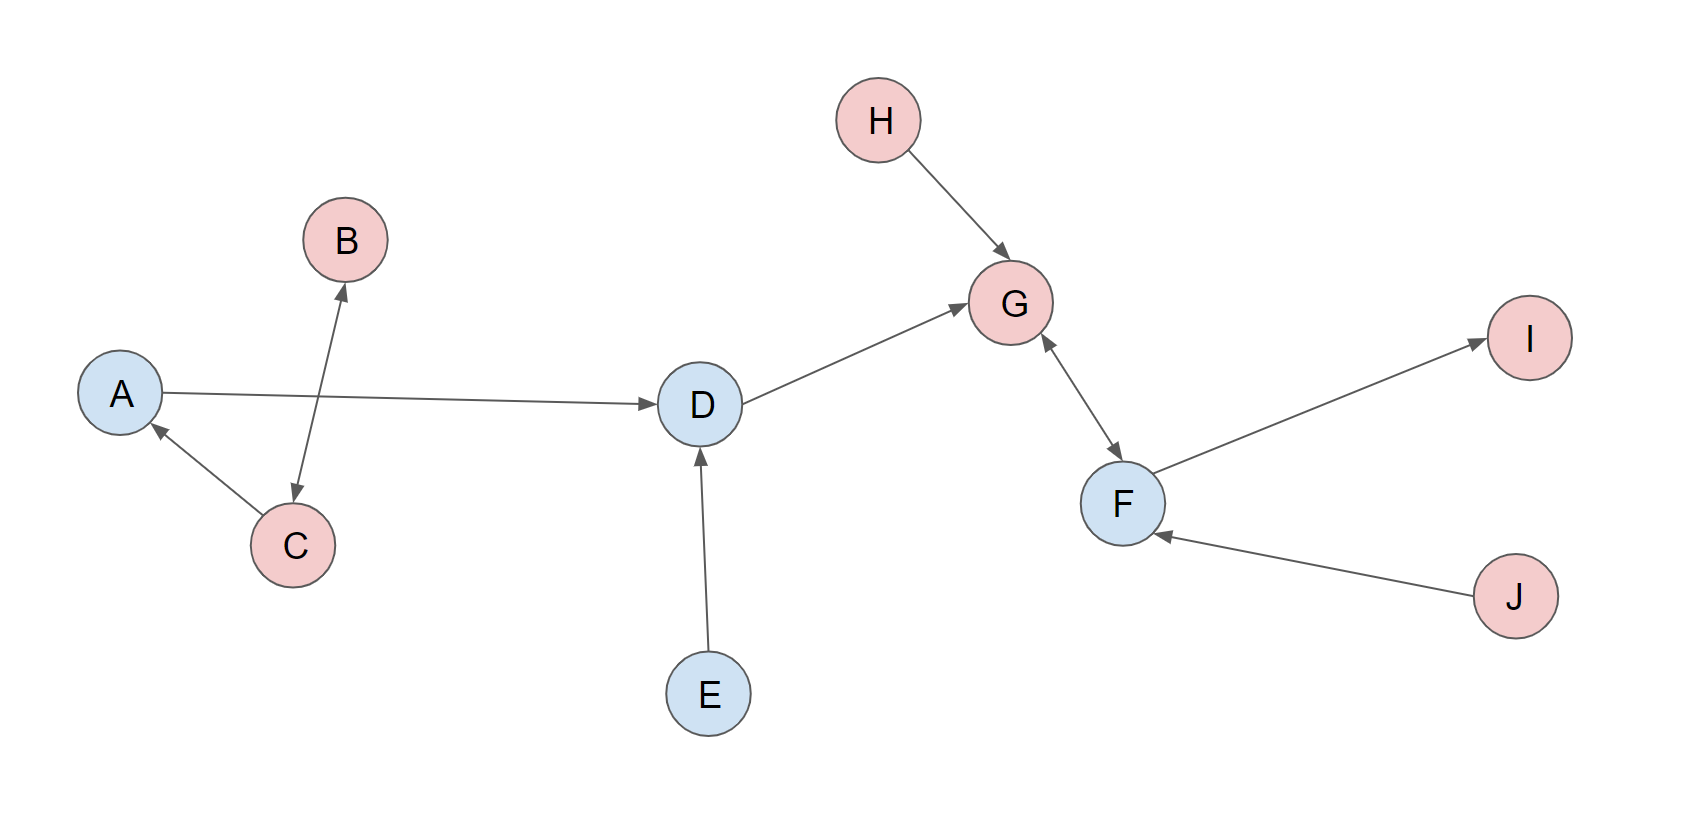
\includegraphics[width=0.7\linewidth]{figures/Networks/Concepts/directed.png} 
        \caption{An example of a network with 10 nodes labeled from A to J. Each node has a color attribute that can be either red or blue. Nodes are connected via directed relationships. Nodes B and C, and nodes G and F have a reciprocal relationship.}
        \label{figure:networkExampleBasic}
    \end{figure}

Graphs provide an abstract representation of the relationships between objects, which may be used to find paths, network flow, connectivity, and more. In this context, we will talk about graphs and networks interchangeably. 

A graph has the following mathematical definition: \label{eq:graph}
    \begin{equation}
        G = (V,E) 
    \end{equation}
Where G is the graph, V is the set of vertices, and E is the set of edges. In figure \ref{figure:networkExampleBasic}, we define G as V = \{A, B, C, D, E, F, G, H, I, J\} and E = \{ \{A,D\}, \{B,C\}, \{C,A\}, \{C,B\}, \{D,G\}, \{E,D\}, \{F,G\}, \{F,I\}, \{G,F\}, \{H,G\}, \{J,F\} \}

\subsection{ Nodes }

A node or vertex is the fundamental element of a network. It is usually represented as a point with lines, known as edges, coming out of it, which connect it with other nodes in the network. Each node represents one elemental object in the network, which in our case is a total of 1038 students. In different contexts, nodes can be cities, computers, or any other concept.

Mathematically, we notate all nodes as V, with each individual node in a graph with lowercase variables, such as x, y, or z. The total number of nodes is notated with $|V|$. In figure \ref{figure:networkExampleBasic}, we have 10 nodes.

\subsubsection{Attributes}

Each node may have different variables, such as sex, BMI, or any other intrinsic variable proper to the object the node is representing. Each of these variables is known as the attributes of a node. Each attribute of a node is notated with subindexes, such as $x_1$, $x_2$, ... , $x_i$ , ... , $x_n$ . In figure \ref{figure:networkExampleBasic}, $A_{color} = blue$

\subsection{Edges}

An edge represents a relationship between two nodes. Our network represents a relationship of undirected friendship. The assessment of friendship is formally introduced in section \ref{method:SocialNetwork}. Two nodes can have multiple edges with the same or different weights between them, or have none. In our case, all weights are equal to one as all relationships are considered of equal value. If all edges in the graph have at least one connection to every other node, then it is called a complete graph.

The mathematical definition of all edges in a graph is as follows:
    \begin{equation}
        E \subseteq  \left\{   (x,y) | (x,y) \in V^2  \land x  \neq y  \right\}
    \end{equation}
We denote the total number of edges as $|E|$. A particular edge between two nodes is simply (x,y). In figure \ref{figure:networkExampleBasic}, we have 11 edges that are directed.

\subsection{Layout}
\label{background:layout}

For visualization purposes, there are several possibilities as to how we can spread the nodes in a typically 2D or 3D image \cite{Fruchterman1991, Kamada1989, osti_1145621, gabor2023, Buja2008}. Proper node placement can help in creating a clear and intuitive picture making it easier to understand the relationships between the nodes. On the other hand, the emerging pattern in the network can be hidden if a poor option is chosen. This is called network layout. In figure \ref{figure:networksLayoutsMDS} we can see an example of all the students and relationships using a \gls{mds} layout \cite{Buja2008}.

    \begin{figure}[ht!]
        \centering
            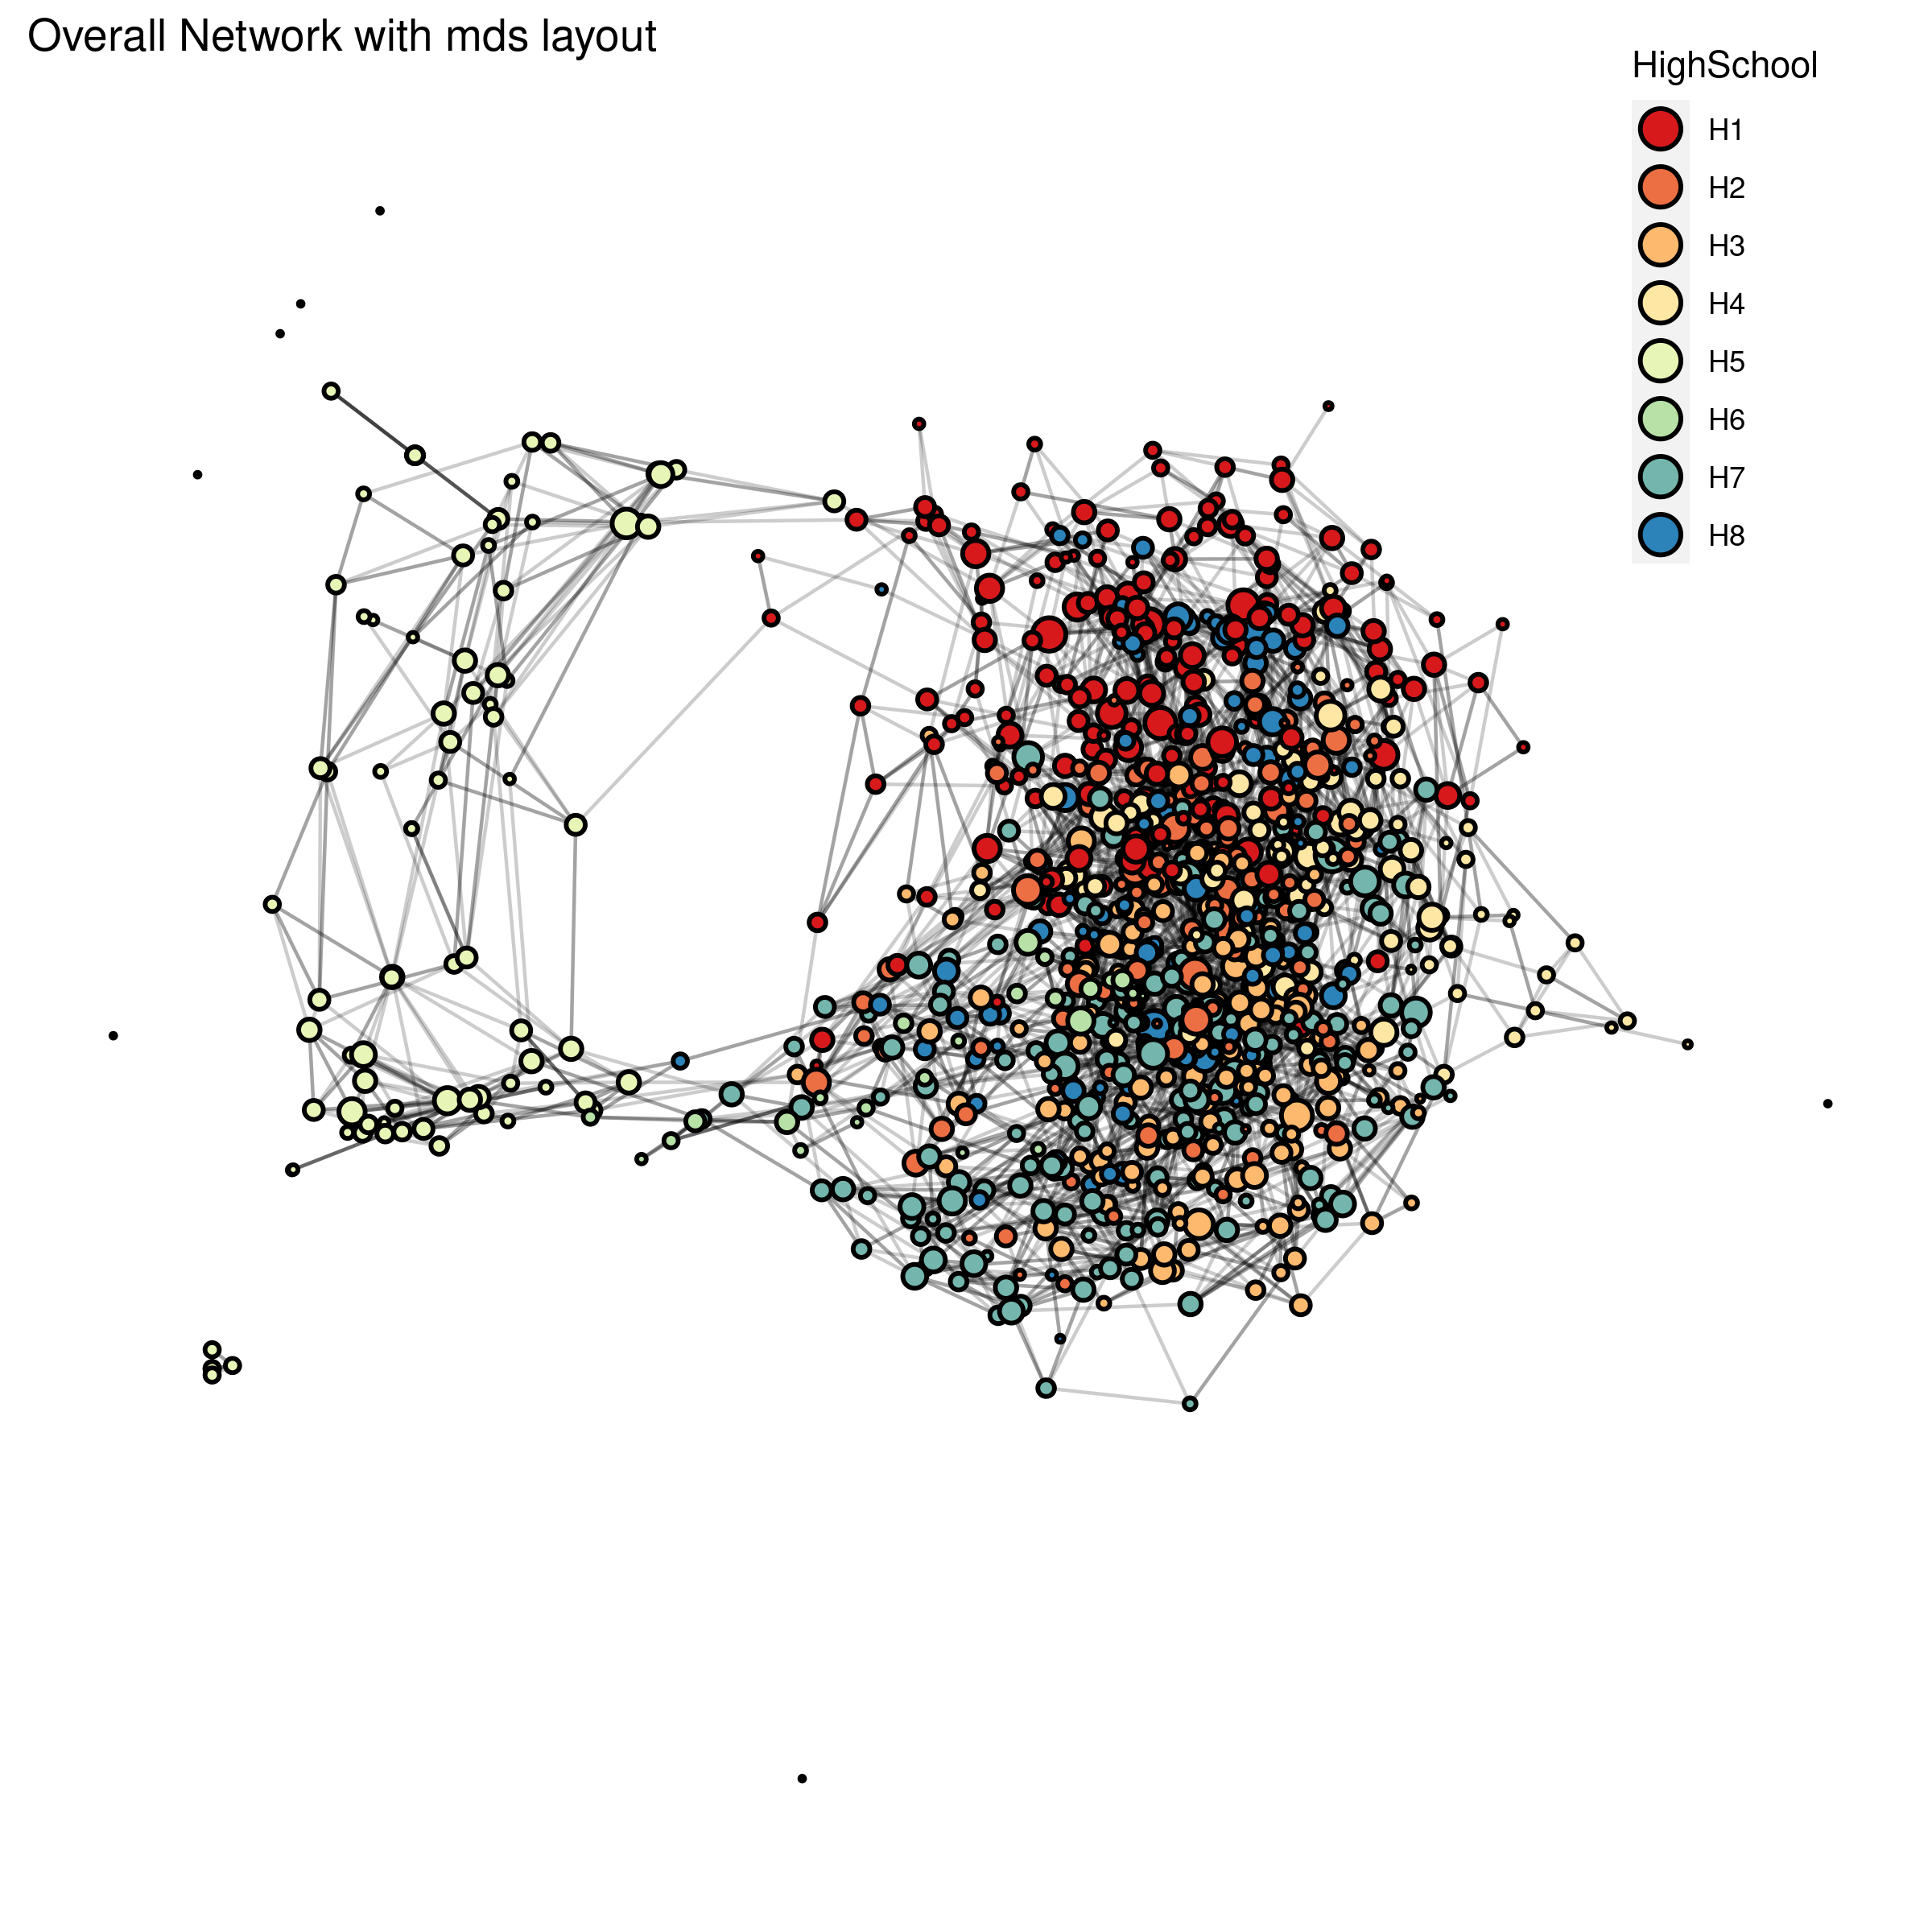
\includegraphics[width=0.9\linewidth]{figures/Networks/Layouts/Graph_OverallNetwork_with_no_highlight_mds_HighSchool___mds.png} 
        \caption{\gls{ff1} overall network with \gls{mds} layout \cite{Buja2008}. Each student is displayed as a node represented as a circle of size proportional to the number of relationships. Each undirected friendship is displayed as an edge represented as a line between nodes. Each node is colored according to the high school to which the student belongs. MDS is a popular dimension reduction technique that tries to maintain similar nodes close to each other.}
        \label{figure:networksLayoutsMDS}
    \end{figure} 


\subsection{Homophily}
\label{network:homophily}

Homophily is the core reason why social network studies work. Individuals tend to form strong bonds with people who are similar to them by factors such as marital status, race, economics, nationality, common interests, and many more \cite{Stehl2013, Moody2001, Qian2007, Cheadle2012, McPherson1987, Sergio2009, Kossinets2009, McPherson2001, Smith2014, Karimi2018, Lee2019, Avin2020, Asikainen2020}. This is also the biggest challenge when interpreting data, as we cannot be sure if individuals who are close to each other are actually influencing each other or simply sharing an environmental factor that influences everyone at the same time to no fault of the nature of their relationships.

Homophily is the ratio of, nodes that have an edge to another node that has the same property, against nodes that have an edge to a node of different property. The homophily value needs to be compared to another homophily value to gain some useful information.

%*****************************************
\section{\textit{Staphylococcus aureus}}
%*****************************************

\subsection{Introduction}

The word "Staphilus" derives from the Greek "σταφυλόκοκκος", composed of "staphylé" meaning bundle, and "coccus" meaning grape. This refers to their bundle of grapes-like arrangement. "aureus" comes from Latin origin meaning golden, which is the golden-orange characteristic color of this bacteria as it is rich in carotenoid pigments. \gls{staph} was discovered in 1880 by Alexander Ogston who noticed a formation of bacteria in pus during a procedure he was performing \cite{Lyell1989}. Wounds caused by \gls{staph} infections were fatal for most patients until the 1940s when it was discovered that benzylpenicillin could cure such infections. But unfortunately, shortly after \cite{Kirby1944}, \gls{staph} evolved into a penicillin resistance strain which became widespread by the end of the century. This led to the development of methicillin \cite{bookstaph} in the 1960s, which was a better option to treat infections caused by the bacterium. However, again, the bacteria evolved to be antibiotic resistant, called \gls{mrsa}. Once this strain was characteristic of the hospital, but today it is widespread (ranging from 2\% to \%80) in both human and cattle population \cite{Shoaib2023}, and thus it is important to understand the \gls{staph} social spread which motivated the writing of \colorbox{PaperColor}{\textcolor{black}{Paper A}}.



% old ref \cite{Prince2012}, why is this bad again?

Nearly 30\% of humans are carriers of \textit{S. aureus} \cite{Kluytmans1997} which are usually present in the skin and the upper respiratory tract. Under normal circumstances the bacteria is harmless, but it can cause a wide range of diseases, ranging from minor skin diseases such as pimples or follicles the most common ones, to life-threatening ones such as pneumonia, endocarditis, and sepsis. \gls{staph} is in the top five most common intrahospital infections and is the most common cause of wound infection after surgery, causing around 500.000 hospital infections in the US alone \cite{Klein2007}, of which 10\% end up in death-related to such infections from the non-antibiotics resistance strain alone \cite{Aratani2021}.

\subsection{\textit{S. aureus} main characteristics}

The mechanisms of the spread of \textit{S. aureus}, as well as the severity of its associated illnesses, are quite diverse. It is important to understand the mechanism of action as well as the vector of infection of any pathogen to evaluate the social impact.

\textit{S. aureus} is a Gram-positive bacterium capable of growing in both aerobic and anaerobic, and a variety of acidic or based places, although it prefers aerobic and neutral acidic environments such as the skin.

The \textit{S. aureus} can have both a capsule and a slime layer depending on the strain. The \textit{S. aureus} capsule inhibits phagocytosis as with many other bacteria capsules. The capsule is prone to contain adhesin proteins which help \textit{S. aureus} adhere to the epithelium of the mucosa, such as skin, nasopharynx, oropharynx, gastrointestinal tract, and in neonates umbilical stump and peri-anal area. The \textit{S. aureus} slime layer is prone to forming biofilms. \cite{Parastan2020}

The peptidoglycan in the cell wall in the \textit{S. aureus} provides surface adhesion proteins that have a very special function. They adhere to the peptidoglycan cell wall (bacteria) and at the same time to fibronectin, fibrinogen, collagen, or elastin (human tissue). Technically, it helps the immune system recognize the bacteria which is why are called \gls{mscramm}. But in the \textit{S. aureus} case \gls{spa} arrest antibodies by binding to the constant part of the \gls{igg}, preventing antibody-mediated immune clearance of the \textit{S. aureus} \cite{Radke2018}. Furthermore, this forms an antigen-antibody complex, which activates the classical complement pathway of the complement immune system, wasting it, and leading to hypocomplementemia which can further aggravate other conditions \cite{Ali2022}.

In \textit{S. aureus}, \gls{clfa} and \gls{clfb} transform fibrinogen into fibrin. They both bind to fibrinogen and promote clotting, forming a shell around the \textit{S. aureus}, which is the way \textit{S. aureus}, a coagulase-positive bacteria that lacks endospores as any other, can actually make something similar to endospores which helps it hide from the immune system in highly localized surfaces \cite{Lacey2019}. This also serves as an adhesion protein that binds the peptidoglycan cell wall to other surfaces and tissues.

\gls{tsst1} is a toxin which can be released by \textit{S. aureus}. This toxin acts as a superantigen. Antigen Presenting Cells have \gls{mhc2} that interact with other cells like T-cells via their CD4 protein. TSST-1 acts as a bridge between the two a hyperstimulates their response leading to a cytokine storm of \gls{il1}, \gls{il2}, \gls{tnfa}, and \gls{ifng}. All of these proteins lead to an inflammatory reaction that acts on the skin creating a rash \cite{Schlievert2021}. They also increase capillary permeability causing vasodilation of the blood vessels leading to both hypotension and hypovolemic shock. Finally, they also increase prostaglandins in the hypothalamus, which leads to fever.

\subsection{\textit{Staphylococcus aureus} diseases}

\gls{staph} is usually harmless and will just colonize the skin and nasopharyngeal tract of the host. However, it is also an opportunistic bacterium that easily attaches to and infects many tissues and can develop much more serious complications there \cite{Berry2022}. These diseases range widely and can be caused by either the bacteria or the toxins produced by them.

Skin lesions include superficial abscesses, folliculitis, furuncles, and carbuncles. Carbuncles can result in generalized sepsis and septic embolisms. \textit{S. aureus} is the most common pathogen associated with wound infections and the most frequently isolated bacteria from chronic wound infections \cite{Bhattacharya2015}. In particular, \gls{ssss} is a skin infection that mainly affects patients with weak immune systems. \gls{ssss} is characterized by blistering of the skin similar to a sunburn-like rash, and the skin may feel like it is scalded, leading to Nikolsky's sign. This last symptom can also be presented as bullous impetigo.

Catheter-associated infections develop from \textit{S. aureus} being attached to medical equipment, forming a biofilm around it, leading to bacteremia \cite{LpezCorts2020}. This can develop further into pyomyositis, endocarditis, lung abscesses, brain abscesses, osteomyelitis, septic arthritis, ocular infections, or necrotizing pneumonia. \textit{S. aureus} can also be introduced into the body due to poor cooking hygiene leading to food poisoning.

Several antibiotic resistant strains exist, such as \gls{mrsa}, \gls{vrsa}, and particularly \gls{lzrsa} \cite{ref:NORMReport, Tsiodras2001, Jones2007, Mendes2008, IkedaDantsuji2011, Seral2011, Mendes2010}.

%*****************************************
\section{Inflammation}
%*****************************************

\subsection{Introduction}

In this study, we want to evaluate if the inflammation response is similar between individuals. Sharing an experiment of copying behaviors among friends can lead to similar immune responses, including inflammation outcomes. This is what motivated the writing of \colorbox{ResultColor}{\textcolor{black}{Result II}}.


Inflammation has 4 main characteristics: heat, pain, redness, and swelling. The combination of these may lead to a 5th one which is loss of function in the affected area. Inflammation is a natural process that the body uses to fight infections and eliminate the cause of inflammation, clear out the area of elements that should not be there, and repair the tissue if damaged. Similar to fever, it has a bad name with the general population even for mild cases despite being a beneficial and necessary process for recovery. People tend to self-medicate in excess with antipyretics and anti-inflammatories which is counterproductive for both healing processes \cite{Serhan2014}. This process of acute inflammation is inherent to the natural healing process of an organism and overall, the natural pathways of inflammation do not pose a risk to the organism's life, and it is counterproductive to interfere with it, as such interference may ultimately impair the healing process in the long run. On the other hand, autoimmune reactions and chronic inflammations are the undesirable form of inflammation that may lead to lasting damage; often in the form of scar tissue.

\subsection{Stimuli}

In order to start an acute inflammation process it is necessary to provide the body with a stimulus, for example, pathogens, toxins, radiation, or physical trauma \cite{LKiss2022}.

\subsection{Clotting}

In the event of an injury, it is imperative to promptly address the issue of bleeding in order to prevent fatality resulting from excessive blood loss.

The first step in blood clotting is the formation of a platelet plug at the injury area. Platelets possess specific receptors on their surface, such as glycoprotein Ib/IX/V, which allows them to adhere to the exposed collagen fibers, resulting in their adhesion to each other and the formation of a temporary seal over the injured site \cite{Li2013}. As platelets aggregate, they release \gls{vwf} so they can stick together, and thromboxane reduces blood flow to the site of injury \cite{ncbibookvmd}. This forms a quick temporal fix that prevents further bacteria from entering the body and provides the basic structure for tissue repair.

Once the platelet plug has formed, a more stable blood clot is formed later on using proteins called clotting factors. These clotting factors work together to convert prothrombin, into thrombin, which in turn converts fibrinogen into fibrin. Fibrin forms a net that reinforces the platelet plug, creating the final stable clot.

\subsection{Acute phase}

Once the clot is in place, it is possible to activate vasodilation and bring in the immune system so it can deal with the infection. Leucocytes have external \gls{prrs} in the cell surface which are activated in contact with \gls{pamps} or \gls{damps}, which trigger the immune and inflammation response \cite{Li2021}. These PRRs are non-specific, meaning that the leucocyte does not know what causes the stimuli, just that something bad is happening and an immune response needs to happen to whatever it is. There is also no cell memory associated with the PRRs.

Additionally, some non-immune cells such as epithelial cells, endothelial cells, and some stromal cells can also express certain types of PRRs that can recognize viral components such as \gls{tlrs} or \gls{rlrs}.

When PAMPs interact with a granulocyte they release histamines, bradykins, and eicosanoids that cause vasodilation in blood vessels and also open a gap in the endothelium releasing blood into the area close to where the DAMP activity is happening, which causes swelling. It also causes muscle relaxation which causes vasodilation (localized hyperemia). You get more blood in the area which turns the area red. It also helps endothelium cells to express more selectins which attract neutrophils to the inflammation site via extravasation (figure \ref{figure:inflammationStarts}). Then neutrophils phagocytose the bacteria. Then dendritic cells present pieces of the bacteria to T-lymphocytes which activates the adaptative immune system if necessary. 

    \begin{figure}[ht!]
        \centering
            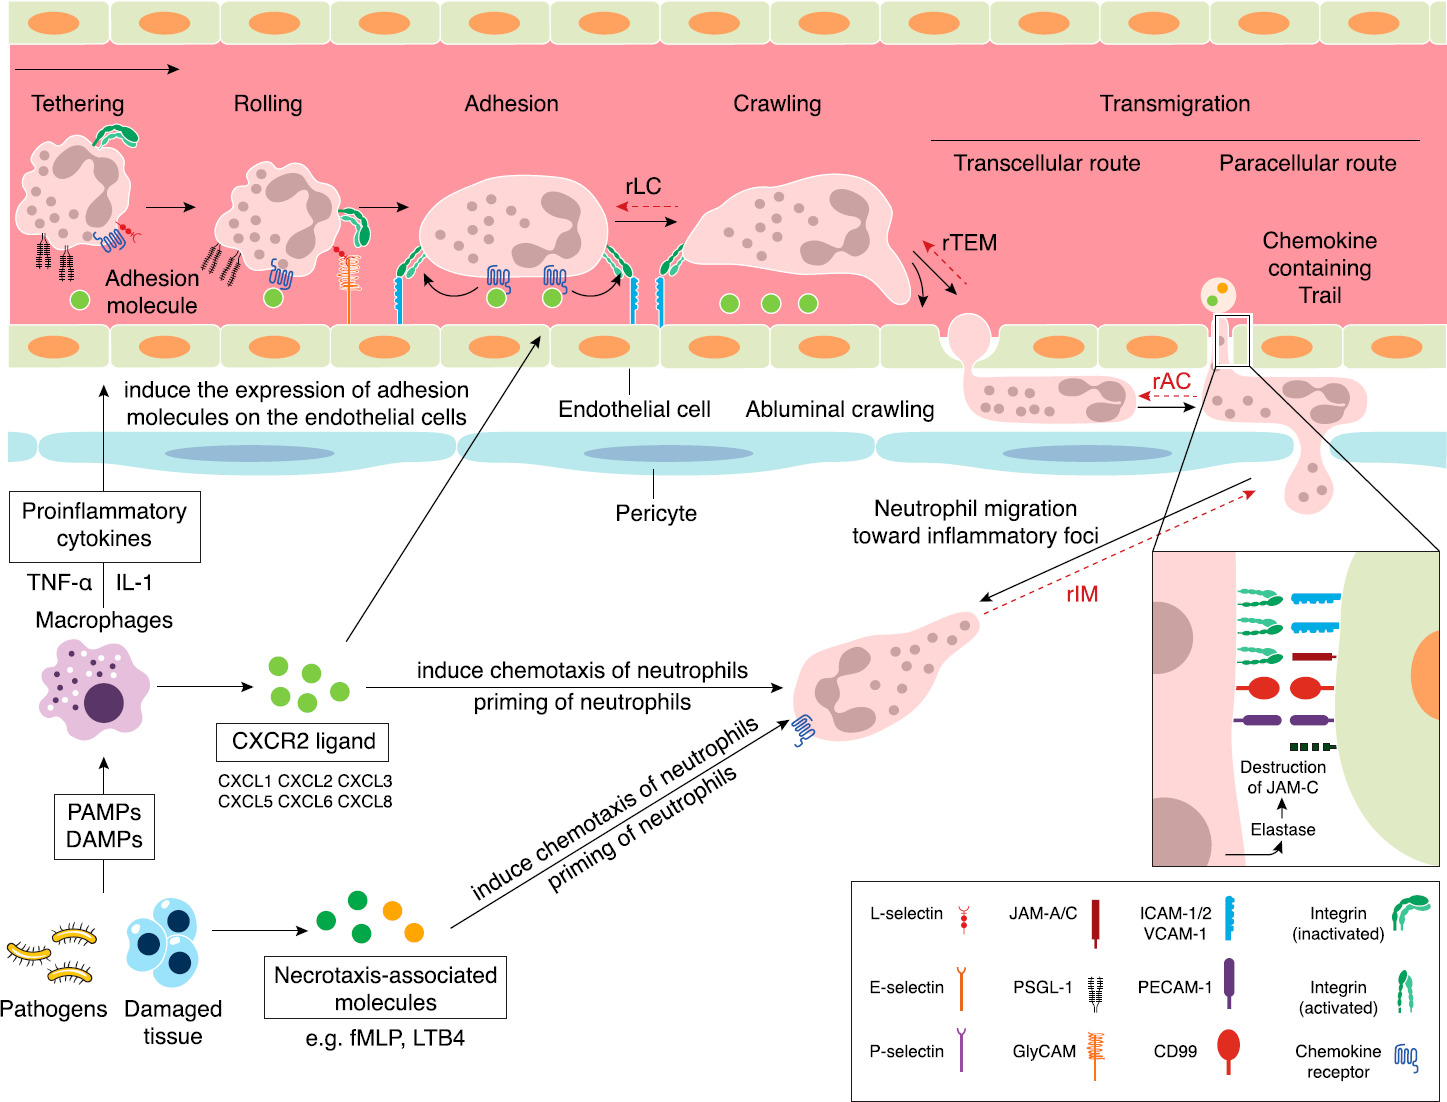
\includegraphics[width=0.8\linewidth]{figures/Inflammation/jlb0617-fig-0002-m.jpg} 
        \caption{Overview of cell migration from a blood vessel to an inflammation site. Image reproduced with permissions from "Deep insight into neutrophil trafficking in various organs" \cite{Hyun2017}.}
        \label{figure:inflammationStarts}
    \end{figure}  

% Permission Order Number: 5656450419799

\subsection{Switching and resolution}

\gls{spm} are produced to inhibit pro-inflammatory mediators and regulate neutrophils. This mechanism is done by the Lipid-mediator-class switching.

Lipoxins reverse the actions of the pro-inflammatory mediators and initiate tissue repair response \cite{Basil2015}. Among many other things, they inhibit chemotaxis, transmigration, superoxide generation, NF-κB activation, generation of pro-inflammatory cytokines, suppress the production of \gls{igm} and \gls{igg} antibodies, reduce the perception of pain due to inflammation, induce the production of elements that neutralize oxidative stress and oxidant-induced tissue damage and block the actions of some leukotrienes. \cite{Sharmawalia2015}

Resolvins play an important role in resolving inflammation by promoting the clearance of cellular debris, bacteria, and other inflammatory mediators. They also inhibit neutrophil recruitment, decrease pro-inflammatory cytokine production, and promote tissue repair and regeneration \cite{Moro2016}. The importance of resolvins lies in their ability to control the duration and intensity of inflammation, which is crucial for preventing the development of chronic inflammatory diseases. They are formed from the metabolism of omega-3 polyunsaturated fatty acids, in particular, \gls{epa} and \gls{dha}. Humans convert \gls{ala} to EPA very inefficiently \cite{Moro2016}, so it is recommended to take food rich in EPA directly such as salmon, mackerel, herring, cod liver, some algae, and human milk. DHA can be converted from EPA but is recommended to also take DHA-rich food such as salmon, caviar, anchovies, mackerel, or herrings.

Protectins reduce inflammation induced by oxidative stress and inhibit the pro-apoptotic signal. Can potentially protect respiratory cells from viral infections. Blocks formation of pro-inflammatory prostaglandins inhibits platelet-aggregating by thromboxane thus blocking the platelet aggregation responses such as those described for \textit{S. aureus}, and stimulate the efferocytosis \cite{Lagarde2014, Serhan2015}.

Maresins (\textit{\textbf{MA}crophage mediator in \textbf{RES}olving \textbf{IN}flammation}) are involved in resolving inflammation and allergic reactions, wound healing, apoptotic human neutrophils by human macrophages, reduced lung inflammation, suppress the production of IL-5 and IL-13, and reduce the production of LTB4 \cite{Serhan2013}.

Eoxins are proinflammatory eicosanoids first described in 2008 \cite{Feltenmark2008} which are suggested to contribute to the inflammation of airways during allergies and some cancers \cite{Claesson2009}. They still have an unknown function in human physiology or pathology. But their production is stimulated in eosinophils by pro-inflammatory mediators \gls{pd2}, \gls{ltc4}, and \gls{il5}.

\subsection{Tissue repair}

Macrophages eat dying or dead cells which provide room for new cells \cite{macrophages2022}. They also secrete growth factors that promote the angiogenesis of temporal capillary vessels. Fibroblasts synthesize collagen in the area of interest. Mild damage in a tissue gets repaired to a normal state, while in severe damage the tissue is replaced by a non-functional fibrous scar.

\subsection{Chronic inflammation}

If everything goes well, the infection has been neutralized, and the inflammation has subsided. However, sometimes errors can occur. Typically this involved not being able to clear the site of inflammation from the cause. For example DAMPs or any other bacterial debris \cite{chronicInfl2016}. In worse cases, external bodies such as undetected wood splints, or metal allocated inside the muscle cannot be removed surgically.

Dysregulation of cytokine signaling can result in excessive production of pro\hyph inflammatory cytokines such as \gls{tnfa} \cite{Li2019}, \gls{il1} \cite{Nouri1984-bv}, or \gls{il6} \cite{Aliyu2022}. Otherwise, a failure or delay of activation of the \gls{spm} mechanisms. Finally, autoimmune diseases such as celiac disease, rheumatoid arthritis, lupus, and many others lead to chronic inflammation.


%*****************************************
\section{Vitamin D}
%*****************************************

\subsection{Introduction}

Vitamin D is crucial in any population, but in the Arctic, it has a special interest due to the lack of sun exposure which limits the availability of this vitamin. If friends share similar vitamin D levels, then it is possible to promote behaviors that enhance vitamin D absorption which motivates the writing of \colorbox{PaperColor}{\textcolor{black}{Paper B}}.


The human body requires what is called essential nutrients, which are compounds that the body cannot synthesize by itself, or is unable to synthesize in large enough quantities. These essential nutrients consist of macro-nutrients, vitamins, minerals, choline, and water \cite{Morris2023-ui}.

Vitamins are organic molecules that the body needs in small quantities for correct metabolism. They are presented in two groups, water-soluble vitamins, and fat-soluble vitamins. Water soluble means they dissolve in water, while fat soluble means that they dissolve in fat. Vitamin D, along with vitamins A, E, and K, belongs to the fat-soluble group, meaning that they are absorbed through the intestinal tract with the help of lipids. Luckily, vitamin D is already present in fat-rich foods such as salmon. Humans need a constant intake of water-soluble vitamins as the body is unable to store them, except for B9 (folate) and B12 (cobalamin) which are not stored either but can last for weeks to years respectively.

There are two primary functions for vitamin D, to absorb calcium and phosphate from the gut into the blood; and to inhibit \gls{pth} production. There are plenty of secondary functions such as immune homeostasis, which showed a worrisome trend during the COVID-19 epidemic in which people with lower vitamin D levels lead by almost 90\% of total deaths \cite{Brenner2020, Dissanayake2021}

\subsection{Sources and metabolism}

There are two methods by which your body obtains Vitamin D, sun exposure (pre-vitamin D3) and food intake or dietary supplements (vitamin D2 and D3) \cite{Bikle2000-yu}. Regardless of intake method, vitamin D needs to undergo two chemical transformations known as hydroxylation to be activated and do its functions. The first one occurs in the liver and transforms vitamin D into \gls{25ohd}, using 25-hydroxylase. This first form of vitamin D is the variable that we measure in the blood serum later on. The second hydroxylation happens in the kidneys and forms \gls{125ohd}, using 1-$\alpha$-hydroxylase, which is the final and physiologically active form of vitamin D. This form is known as calcitriol. If calcitriol becomes excessive, then is converted to 24,25-dihydroxycholecalciferiol, which is less active. This prevents hypervitaminosis D, and it is why this condition is very rare \cite{Holick1995} unless a person takes an overwhelming amount of vitamin D supplements \cite{MarcinowskaSuchowierska2018}.

Both vitamins D2 (ergocalciferol) and D3 (cholecalciferol) raise 25(OH)D levels. The metabolism and actions of vitamins D2 and D3 are identical, and they only differ in the chemical morphology present in their side-chain structure. Evidence suggest that vitamin D3 increases 25(OH)D levels greater and longer than vitamin D2 \cite{ref:Tripkovic2012, ref:Lehmann2013, ref:Logan2012, ref:Tripkovic2017}. Dietary supplements of 25(OH)D3 are three to five times as potent as vitamin D3 supplements \cite{ref:GraeffArmas2019, ref:QuesadaGomez2018}. In any case, all form of dietary vitamin D is absorbed in the small intestine via passive diffusion using intestinal membrane carrier proteins \cite{ref:Silva2017}. As stated before, the presence of fat helps the diffusion and absorption of vitamin D, although some vitamin D can still be absorbed without fat.

\subsection{VDR}

Lastly, calcitriol needs to enter the cells; this is where the \gls{vdr} comes into play. This protein is mostly found in the cells of the small intestine, immune system, kidneys, and bones. Calcitriol then binds to VDR, which forms a protein complex that enters the nucleus of cells and binds to DNA, up or down-regulates the expression of hundreds of genes \cite{Nagpal2005, Dusso2005}. This includes calcium absorption (promotes calbindin), bone formation, cell growth \cite{Samuel2008}, and immune function. VDR regulates the production of cytokines in the immune system, generally acting as an anti-inflammatory agent, facilitating humoral response, and leading to homeostasis. In figure \ref{fig:vitVDRimmune} we see an overview of these functions.

\begin{figure}[ht!]
{
    \centering
    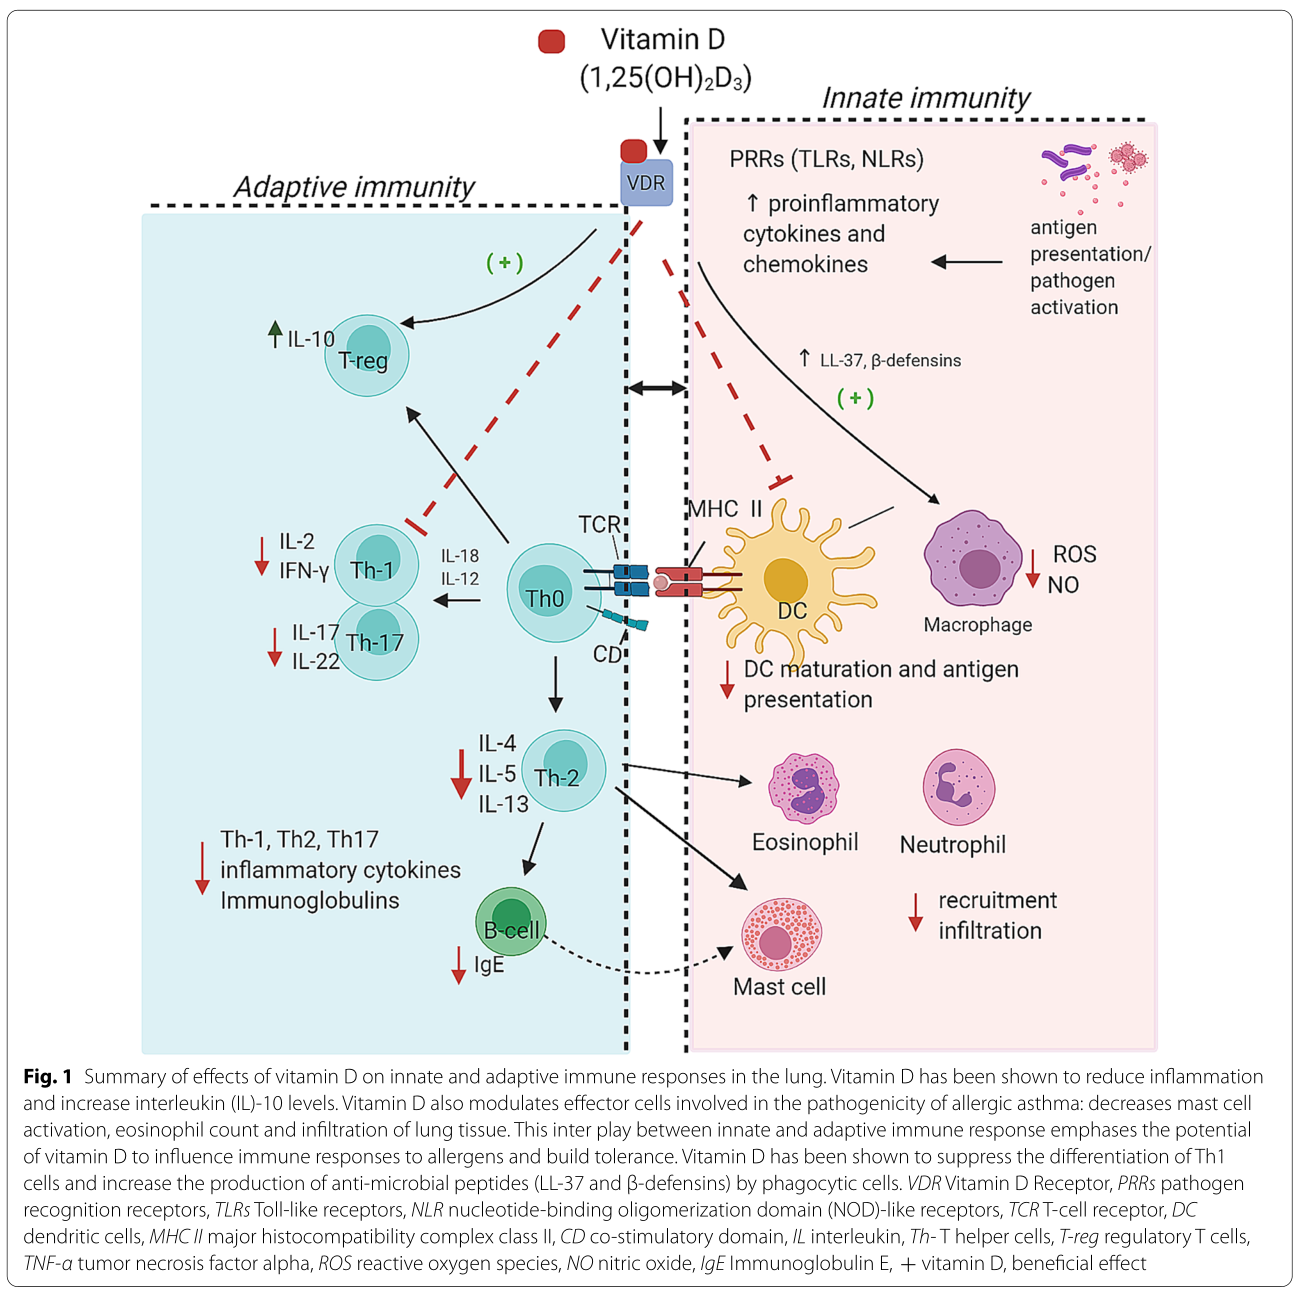
\includegraphics[width=1\textwidth]{figures/Vitamin D/VDRImmunity.png}
    \caption{Vitamin D effects on the immune system. Figure reproduced under CC4.0 license from "Recent advances in vitamin D implications in chronic respiratory diseases" \cite{Gaudet2022}.} 
    \label{fig:vitVDRimmune}
}
\medskip
\end{figure}


%*****************************************
\section{Over-the-counter medicine}
%*****************************************

\subsection{Introduction}

\gls{otc} medicine \cite{Algarni2021} refers to a type of medication that is sold without the need for a prescription and can be acquired even outside of pharmaceutical outlets such as supermarkets. These types of medicine have a low dosage of the active agent and are used to alleviate common symptoms such as pain, fever, cough, allergies, and digestive issues

\gls{otc} are fairly safe when used in moderation and responsibly. However, this is not always the case. About 16\% of the population misuse these medicines, and up to 7\% are addicted to them \cite{Algarni2021, ijerph18115530, PolandSelfMedicate, Lein2023}. Common reasons for its use are the false belief that if taken more the symptoms will go away faster, or to the contrary, for self-harming purposes \cite{Algarni2021}. In Norway \cite{Lorentzen2018}, teenagers report using these drugs mostly for physical pain, to alleviate stress and fatigue, due to familiar conflicts, and to appear socially successful; while the common user is a person with constant pain, binge drinking, having school problems, bad sleeping habits, lower life ambitions and high spare time. About 55\% of \gls{otc} medicines are sold in non-pharmaceutical outlets \cite{Lorentzen2018}.

In this section, a short summary of common \gls{otc} medicines will be listed in addition to their function, mechanism of action, possible side effects, and how they are used as recreational drugs \cite{otcAbuse2020}.

\subsection{Analgesics}

Analgesics are a class of drugs commonly known as painkillers. They reduce or block the perception of pain signals in the brain. \gls{nsaids} usually overlap their effect with analgesic medicine but will be discussed in the antiinflammatories section.

The most common active component of analgesics is paracetamol (acetaminophen) \cite{Brune2014}. This is metabolized in the liver and flushed into the kidney fairly quickly. About 2\% of it transforms into \gls{napqi}, which remains in the liver for a longer time before it also moves into the kidneys. However, \gls{napqi} is toxic. When taken in a low amount, the liver can detoxify \gls{napqi} quickly enough before it becomes a serious problem by combining it with a molecule called glutathione. Problems arise when analgesics are taken in higher doses or at a higher frequency, the liver may become overwhelmed and unable to detoxify all of the \gls{napqi}, leading to liver damage and potentially liver failure.

In contrast, non-OTC analgesics are usually opioids such as morphine. They work by binding to specific receptors in the brain and spinal cord called opioid receptors \cite{Schulz2004}. Activating these receptors blocks the transmission of the most severe pain signals. However, they are at risk of addiction and their use is severely restricted.

Analgesics are not used as recreational drugs directly but are used in combination with other substances such as alcohol or cannabinoids \cite{otcAbuse2020}.

\subsection{Antihistamines}

Antihistamines are a class of medications that are commonly used to treat allergic rhinitis and allergic-like symptoms. They work by blocking histamine, hence their name. Histamine is released when allergens bind to mast-cell-bound \gls{ige} antibody sites \cite{Vardanyan2016}. This is commonly known as an allergy and is the mechanism of bronchial smooth muscle contraction, urinary bladder contractions, vasodilation, visceral hypersensitivity, itch perception, urticaria, sneezing, hyper-secretion from glandular tissue, and  nasal congestion due to vascular engorgement.

Different antihistamine medications can cause both vasoconstriction and vasodilation. In general, vasodilation may be more effective at relieving symptoms such as congestion and mucus production, while vasoconstriction may be more effective at reducing inflammation and swelling. But both cases can be detrimental. Vasoconstriction can increase blood pressure in the heart and reduce blood flow in the kidneys. For patients with decreased kidney functionality or hypertension, this would be dangerous. Vasodilation increases blood flow, which is generally beneficial for normal kidney function. However, it is detrimental in cases when the patient is incapable of filtering waste, and excess fluid from the blood would lead to a buildup of toxins and fluid in the body. Lastly, worth mentioning that the first generation of antihistamines developed during the 1930s have a detrimental flaw and they tend to cross the brain-blood barrier \cite{Walsh2005}. The blood-brain barrier is a specialized system of blood vessels that helps to protect the brain from harmful substances and toxins.

The effects of drug abuse related to antihistamines have a huge variety, but as a general rule, they are used as vasodilators, which promote a calming and sedating effect. They can enhance the effect of other substances such as making opioids more hallucinogenic, especially the first generation \cite{otcAbuse2020}.

\subsection{Antiinflammatories}

\gls{nsaids} drugs such as ibuprofen work by inhibiting the production of prostaglandins. Prostaglandins cause blood vessels to dilate, which can increase blood flow to the affected area and cause redness and swelling. They also sensitize nerve endings to pain, which can cause pain and discomfort. NSAIDs work by inhibiting the activity of an enzyme called \gls{cox}, (subdivided into COX1 and COX2) which is responsible for the production of \gls{pg} \cite{Faki2021}.

NSAIDs can be divided broadly into three categories, COX1 inhibitors, COX2 inhibitors, and both COX1 and COX2 inhibitors. Prostaglandins PGE2 and PGI2 participate in the synthesis of protective mucus and gastric flow, which is why a normal side effect of COX1 inhibitors is gastrointestinal bleeding and ulcers \cite{Faki2021}. COX1 also participates in the production of thromboxane which promotes platelet aggregation, which is why antiinflammatories such as aspirins can cause an increase in bleeding. On the other hand, prostaglandins PGI2 and PGH2 are vasodilators and share COX precursors with thromboxane which is also a vasoconstrictor. Simply put, there must be an equilibrium between COX1 (vasoconstrictor) and COX2 (vasodilator). NSAIDs that inhibit COX2 increase blood pressure which can lead to heart infartion \cite{Faki2021}. These side effects can be mitigated with the usage of prostaglandin analog medicines.

Due to their vasoconstriction nature, these medicines can be used as stimulants, which can also induce psychotic symptoms, paranoia, and visual hallucinations. \cite{otcAbuse2020}

\subsection{Cough syrups}

Cough syrups are used to stop unwanted coughing which may cause discomfort, or even physical injuries, in the upper respiratory tract. Their mechanism of action is not fully understood but their effects are accomplished by reducing the signaling between the laryngeal nerves and vagus nerve \cite{Bardal2011}.

The three main antitussive components are codeine, \gls{dxm}, and benzonatate \cite{Beharry2016}. Codeine breaks down into codeine-6-glucoronide and morphine, which stimulates the µ-opioid receptors \cite{Schulz2004} causing euphoria, constipation, and also cough suppression. \gls{dxm} in the principal component in \gls{otc} medicines, and it has similar side effects of codeine but in the form of hallucinogenics, and in particular as a dissociative. Benzonatate is a non-narcotic drug that works as a local anesthetic in the whole respiratory tract. 

Due to their action on the peripheral nervous system, the main side effect of these drugs is reduced consciousness in the form of drowsiness. In higher dosages, it can lead to hallucinations, paranoia,
perceptual distortions, delusional beliefs, ataxia, and out-of-body experiences \cite{otcAbuse2020}.

\subsection{Antidiarrheals}

The main component of these drugs is loperamide. Loperamide works by binding to peripheral µ-opioid receptors in the gastrointestinal tract \cite{Malinky2021}. It inhibits the release of acetylcholine and other neurotransmitters that stimulate the contractions of the intestinal wall. This leads to a decrease in the motility of the intestines, which slows down the passage of stool and reduces the frequency and urgency of bowel movements. This also allows for the gastrointestinal tract to have more time absorbing fluids, increasing the hardness of the fecal matter.

Similar to antitussive medications, antidiarrheals relax the peripheral nervous system. Thus, these drugs are used also as opioids, to alleviate symptoms of opioid withdrawal, or as a psychoactive. \cite{otcAbuse2020}

%*****************************************
\section{Machine learning}
%*****************************************

\subsection{Introduction}

\gls{rf} and \gls{anns} are both popular machine-learning algorithms used for classification and regression tasks \cite{AlZaiti2022}. RF combines multiple decision trees to make predictions, and ANNs simulate the behavior of neurons in the brain. RF randomly selects a subset of input features for each tree, whereas ANNs use all input features available in the data. RF is more straightforward to interpret than ANNs, which have more complex interconnections and act more like a black box model. However, ANNs can reproduce better complex and non-linear relationships between input features. RF is prone to overfitting. ANNs share the same problem if the model is too complex or the training data is not large enough. ANNs also require tuning various hyperparameters to achieve a good prediction rate.

There are other classical machine learning techniques which could be applied. Support Vector Machines (SVM) \cite{AlZaiti2022} are also good with high non-linear dimensional data and have good generalization, but are computationally intensive and in particular difficult to interpret and visualize. K-Nearest Neighbors (KNN) \cite{AlZaiti2022} could be potentially used to classify subjects into different strategies, each being the optimal strategy for achieving healthy weight (i.e.: Smoking less, having more friends, etc.), but it goes a bit beyond our objective of trying to explain what influenced a person's BMI value the way it is. Naive Bayes is very simple, quick, and  easy to interpret, but it assumes independence between variables which in our case is too much of a stretch in the assumptions. Gradient boosting can be used in future work when we lay out the basics for our models. ANN and RF were finally selected as the most relevant models for \colorbox{ResultColor}{\textcolor{black}{Result III}}.



\subsection{Interpretability}

An important concept is the interpretability aspect of the machine learning models \cite{Somani2023}. It is crucial as machine learning is increasingly being used in critical areas such as healthcare, finance, and law where clear explanations are essential.  In general, methods offer easy interpretability in exchange for lower accuracy. The key concept in our context is feature importance, which aims to identify the variables that have the most influence on the model's predictions. For example, it's important to identify which variables are most important for predicting the risk of heart disease; variables such as age, blood pressure, and cholesterol levels may be more important than gender, BMI, or occupation. 

\subsubsection{SHAP values}

\gls{shap} computes Shapley values \cite{NIPS2017_7062}, which is a mathematical concept from Cooperative Game Theory, to explain the contribution of each input feature to the final prediction of the model. SHAP can be used on any machine learning algorithm and is easy to interpret, but it requires a large number of samples to properly capture the interactions of variables. RF in particular has the advantage of having a very easy-to-interpret model.

\subsubsection{Mean Decrease in Impurity}

\gls{mdi} \cite{Breiman2001} is a measure used in random forests to quantify the importance of each feature in predicting a target variable. The MDI is calculated by measuring the importance of each variable, in each tree, and calculating how the impurity is reduced. When a variable is used to split a tree node, it reduces the impurity of that node, and the reduction in impurity correlates to the importance of that variable. The MDI for a feature is calculated by averaging the reduction in impurity across all trees in which that feature is used. Higher MDI means more importance.

\section{Statistical Analysis}

\subsection{Contingency tables and Pearson $X^2$ test}

Contingency tables are used to determine if the total number of samples in a combination of two categorical variables (i.e.: Sex and BMI), happens to be within the range of the values that we would expect by chance \cite{Bonamente2022}. Several tests can be performed to determine if these combinations are suspicious or not. One in particular is the Pearson Chi-square test which uses a Chi-square distribution for a specific degree of freedom. The degree of freedom is related to the number of variables in the calculation and they represent the number of independent pieces of information available to estimate or calculate statistics. The Chi-square value is calculated by taking the sum of the squared differences between the observed and expected data, dividing by the expected data, and then multiplying that result by the number of variables. The resulting value is compared to the values in the Chi-square table to determine if the null hypothesis can be rejected or not.

If the p-value of the analysis is significant, it means that some combinations of variables are suspiciously high or low. Each combination can, later on, be tested using a simple binomial test to highlight values far away from the expected ones.

\subsection{Logistic regression}

Logistic regression is a type of statistical analysis used to predict the probability of an event occurring based on a set of variables \cite{Bewick2005}; in our case, we use many results to tell what the probability of a subject having an effect as the number of friends increases or decreases. Is named after the logistic function which takes an S-shaped curve that can take any input value and map it to a value between 0 and 1, representing the probability of an event occurring. It is primarily used when the dependent variable is categorical or binary, such as yes/no, true/false, or success/failure.

In logistic regression, the odds ratio tells us how much more likely it is for the dependent variable to occur compared to not occurring, given a change in the independent variable. Probability and odd ratio are not directly interchangeable because they have different scales and have a non-linear relationship, but they can be approximated by:
\begin{equation}
    Probability = odds / (1 + odds)
\end{equation}

\subsection{Autocorrelation models}

An autocorrelation model is a statistical model that measures the relationship between a variable and its past values. This technique is commonly used in time-series analysis to identify patterns and trends over time \cite{anselin1988spatial}. In the context of network analysis, these models \cite{OMalley2008} strive to find how a network has changed until it finds an equilibrium point at the current time. We aim to find the ρ coefficient in the formula:
    \begin{equation}
        Y(t+1) = ρW_nY(t) + Xβ + ε
    \end{equation}
W is a weighted matrix of friends, which indicates who influences whom. X is the explanatory variable (sex, BMI, smoke...), and β is a vector of coefficients the same as in regular linear regression. Symbol ε is a random error noise vector. Y is the dependent variable vector which varies over time (t). This equation converges to a common value as t is increased. The ρ coefficient represents how much importance has the influence of friends, which ranges typically from 0 to infinity although negative values are also valid depending on the context. A value close to 0 would mean that friends have no influence. Negative values would indicate that friends influence others into doing the complete opposite, which could make sense for example if the explanatory variables are mutually exclusive and encoded with dummy variables.